\documentclass[14pt,letterpaper]{article}

\newcommand{\IncludePath}{../include}
\usepackage{extsizes}
\usepackage{titling}

\usepackage{amssymb,amsmath,amsthm}
\usepackage{enumerate}
\usepackage[margin=1in]{geometry}
\usepackage{graphicx,ctable,booktabs}
\usepackage{fancyhdr}
\usepackage[utf8]{inputenc}

\makeatletter
\newenvironment{problem}{\@startsection
       {section}
       {1}
       {-.2em}
       {-3.5ex plus -1ex minus -.2ex}
       {2.3ex plus .2ex}
       {\pagebreak[3]
       \large\bf\noindent{Problem }
       }
       }
\makeatother

\pagestyle{fancy}
\lhead{\thetitle}
\chead{}
\rhead{\thepage}
\lfoot{\small\scshape Grade 4 Olympic Math}
\cfoot{}
\rfoot{}
\renewcommand{\headrulewidth}{.3pt}
\renewcommand{\footrulewidth}{.3pt}
\setlength\voffset{-0.25in}
\setlength\textheight{648pt}
\setlength\headheight{15pt}


\title{Angles I}
\author{Name: \underline{\hspace{5cm}}}
\date{October 1, 2016}

\begin{document}
\HomeworkTitle

\thispagestyle{empty}

\begin{problem}{Unit Conversion}
  Recall that \begin{itemize}
    \item $\SI{1}{\kilo\metre}=\SI{1000}{\metre}$
    \item $\SI{1}{\metre}=\SI{100}{\centi\metre}$
  \end{itemize}
  Using this information, what is \SI{3}{\kilo\metre} converted to centimetres?
  \hfill \blankE \si{\centi\metre}
\end{problem}

\begin{problem}{Acute, Right, Obtuse}
 Circle the correct category for each angle.

 \begin{itemize}
  \item \SI{123}{\degree} \hfill Acute~~Right~~Obtuse
  \item \SI{88}{\degree} \hfill Acute~~Right~~Obtuse
  \item \SI{90}{\degree} \hfill Acute~~Right~~Obtuse
 \end{itemize}
\end{problem}

\begin{problem}{Angle sum}
 \begin{itemize}
  \item The sum of an acute angle and a right angle is:
        \hfill Acute~~Right~~Obtuse
  \item Half of a right angle is:
        \hfill Acute~~Right~~Obtuse
 \end{itemize}
\end{problem}

\begin{problem}{Triangle angle sum}
 The sum of the angles of a triangle is \SI{180}{\degree}. Two of the angles
 measure \SI{25}{\degree} and \SI{140}{\degree}. What does the third angle
 measure?
\end{problem}

\begin{problem}{Supplementary}
 Two angles are supplementary. One is \SI{20}{\degree} greater than the other.
 Find both angles.
\end{problem}

\begin{problem}{Lines I}
 Five lines are on a plane. No two lines are parallel, and no three (or more)
 lines intersect at a single point. How many points on the plane lie on more
 than one line?
\end{problem}

\begin{problem}{Lines II}
 Find two rays that do not intersect, but if each ray is extended to a line,
 then the resulting lines do intersect. (``Extending'' a ray to a line means
 continuing the ray from its endpoint, but in the opposite direction of the
 ray. The resulting object extends infinitely in both directions, and so is a
 line.)
\end{problem}

\begin{problem}{Challenge}

\begin{wrapfigure}{r}{0pt}
 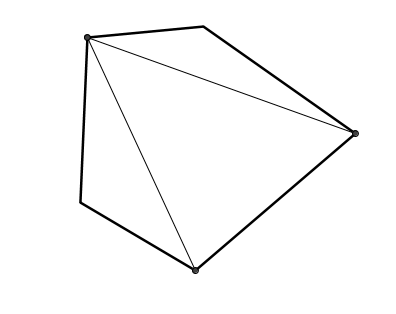
\includegraphics[width=10em]{pentagon.png}
\end{wrapfigure}

The sum of the interior angles of a triangle is \SI{180}{\degree}.

\begin{enumerate}
 \item What is the sum of interior angles of a rectangle?
 \item Use the picture to show that the sum of interior angles of any pentagon
 is \SI{540}{\degree}.
 \item Draw an octagon (eight-sided shape). What is the sum of its interior
 angles?
 \item When one side is added to a shape (for example, changing a triangle
 [$3$] to a quadrilateral [$4$]), by how much does the angle sum change? Why?
\end{enumerate}

\end{problem}

\end{document}
